16. \begin{figure}[ht!]
\center{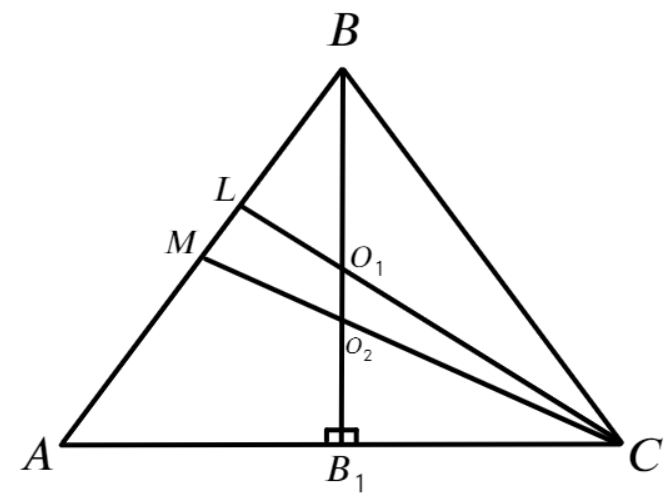
\includegraphics[scale=0.35]{g9-16.png}}
\end{figure}\\
Пусть $CL$ биссектриса, $CM$ медиана, а $BB_1$ --- и то, и другое. По теореме Пифагора $BB_1=\sqrt{5^2-3^2}=4.$ Так как медианы делятся точкой их пересечения в отношении $2:1,$ имеем $O_2B_1=\cfrac{1}{3}\cdot4=\cfrac{4}{3}.$ По свойству основания биссектрисы имеем $\cfrac{BO_1}{B_1O_1}=\cfrac{BC}{CB_1}=\cfrac{5}{3},$ откуда $O_1B_1=\cfrac{3}{8}\cdot4=\cfrac{3}{2}.$ Таким образом, $O_1O_2=B_1O_1-O_2B_1=\cfrac{3}{2}-\cfrac{4}{3}=\cfrac{1}{6}.$\\
